\documentclass[11pt,a4paper]{article}
\usepackage[utf8]{inputenc}
\usepackage[T1]{fontenc}
\usepackage{array}
\usepackage{amsmath}
\usepackage{amsfonts}
\usepackage{siunitx}
\usepackage{placeins}
\usepackage{amssymb}
\usepackage{makeidx}
\usepackage{sidecap}
\usepackage{fvextra}
\usepackage{multicol}
\usepackage{listings}
\usepackage{appendix}
\usepackage{comment}
\usepackage{nicematrix}
\usepackage{multirow}
\usepackage{braket}
\usepackage{graphicx}
\usepackage{relsize}
\usepackage{fancyhdr}
\usepackage{cprotect}
\usepackage{color} 
\usepackage{hyperref}
\hypersetup{
	colorlinks=true, 
	linktoc=all, 
	linkcolor=blue,
	urlcolor=blue
}
\usepackage[left=2cm,right=2cm,top=1.5cm,bottom=2cm]{geometry}
\usepackage{titling}
\usepackage{etoolbox}
\flushbottom
\title{Statistical Analysis of Experimental Data\\
	\vspace{0.2cm}
	\large{Homework 01}}
\vspace{-0.2cm}
\author{Igor Di Tota}
\date{\small \url{https://github.com/igordt/SAED_homeworks/tree/main}}


\begin{document}
	\maketitle
	
	\section*{Introduction}
	
	The data set used in this homework is provided by the OECD and contains the population of Poland for every year from 1950 to 2025.
	For each year, the number of people is given separately for men and women and for different age categories.
	
	As a first overview, Figure~\ref{fig:total} shows the total population of Poland as a function of the year of measurement.
	The population grows from about $24.8$ million in 1950 to a maximum of about $38.5$ million in 2012, and then slowly decreases to $37.4$ million in 2025.
	
	\begin{figure}[!h]
		\centering
		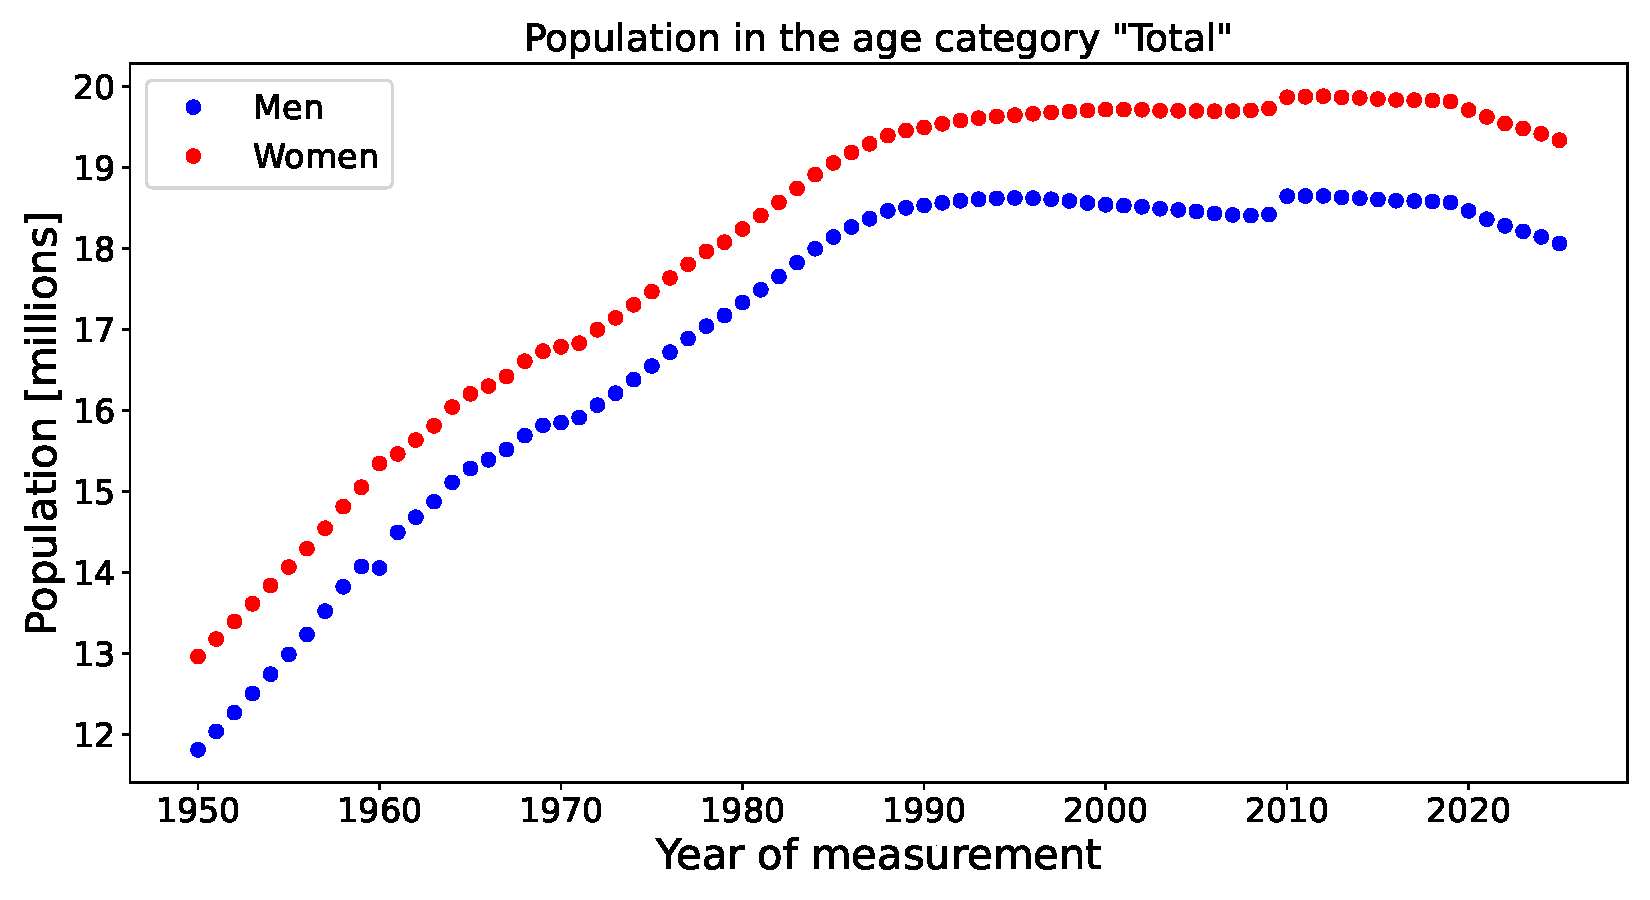
\includegraphics[width=0.9\linewidth]{images/_T.pdf}
		\caption{Total population of Poland for men and women as a function of the year.}
		\label{fig:total}
	\end{figure}
	\FloatBarrier
		
	To better understand the structure of the data, the age categories were examined.
	The data set contains 24 categories, present in every year, which can be divided into two types:
		\begin{itemize}
		\item \textbf{18 five-year age groups}, which do not overlap: $0$--$4$, $5$--$9$, \dots, $80$--$84$ years, and $85$ years or over
		\item \textbf{5 aggregate categories}, obtained by summing several five-year groups:
		\begin{itemize}
			\item less than 20 years
			\item $15$--$64$ years
			\item $20$--$64$ years
			\item 50 years or over
			\item 65 years or over
		\end{itemize}
		\item \textbf{the total population}.
	\end{itemize}
	
	The object of this homework is the group of people born in 1946--1950, who in 1950 were not older than 4 years and therefore belong to the age group $0$--$4$.
	Since the age groups are five years wide, after five years the same people are found in the next age group.
	In the years
	\begin{equation}
		t_k = 1950 + 5k, \qquad k = 0, 1, \dots, 15,
	\end{equation}
	they belong to the age group $5k$--$(5k+4)$ years.
	The last available year, 2025, corresponds to $k = 15$ (age group $75$--$79$), so the group can be followed at 16 points in time.
	
	This is shown in Figure~\ref{fig:age_structure}, where the age distribution of Poland is plotted for four different years.
	The group of our interest highlighted in red.
	
	\begin{figure}[!h]
		\centering
		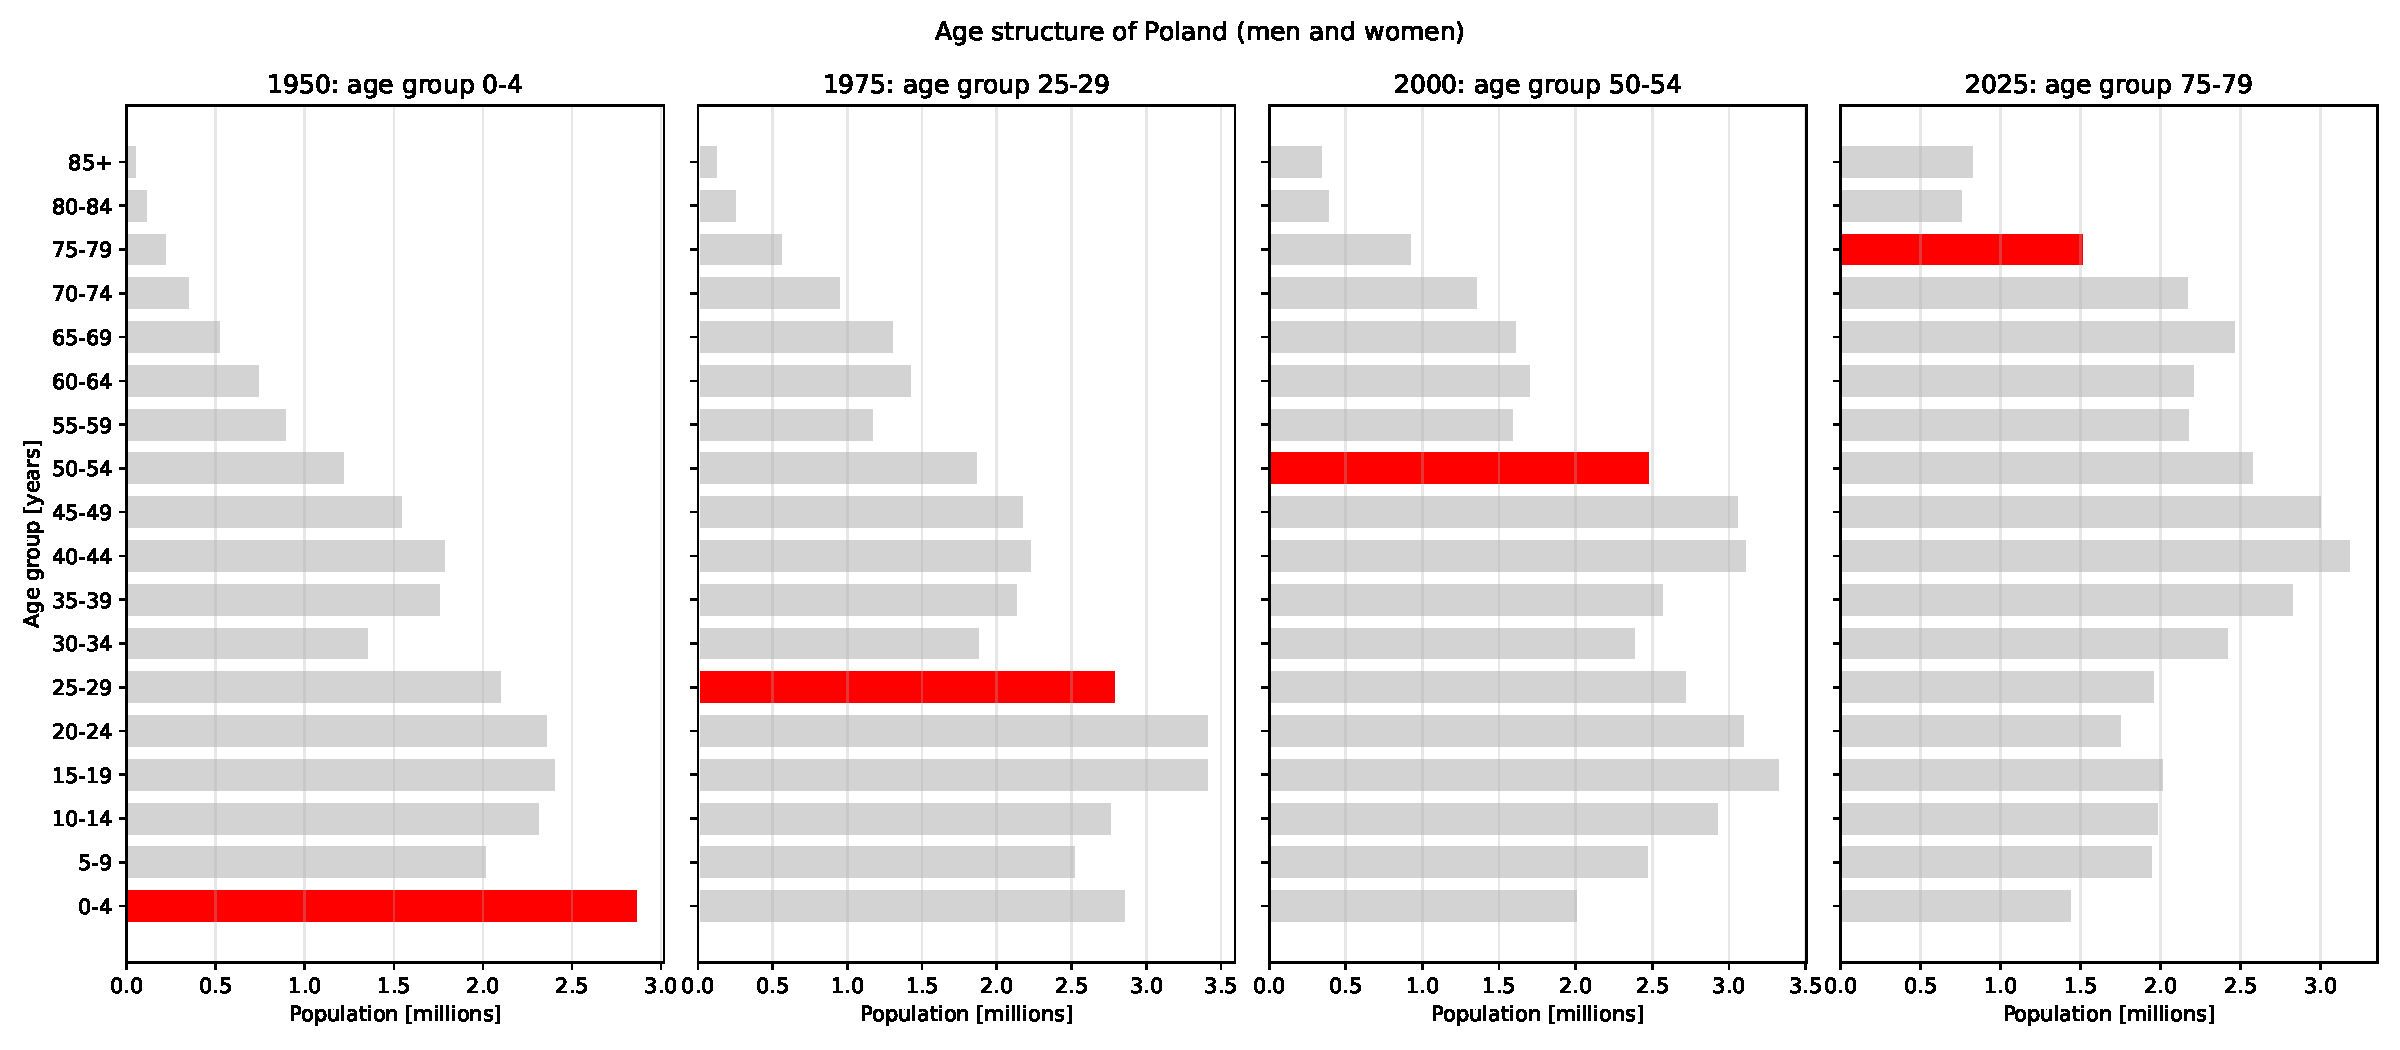
\includegraphics[width=\linewidth]{images/age_structure.pdf}
		\caption{Age distribution of Poland (men and women) in 1950, 1975, 2000 and 2025. The age group containing the people born in 1946--1950 is shown in red.}
		\label{fig:age_structure}
	\end{figure}
	\FloatBarrier
	
	\section*{Task 1}
	
	\textit{Prepare the plot showing the population of men and women born in 1946--1950 (not older than 4 in 1950), as a function of year (or age).}
	
	\vspace{0.2cm}
	
	For each $k = 0, \dots, 15$ the population of men, $N_M(t_k)$, and of women, $N_F(t_k)$, is selected from the data set for the year $t_k$ and the age group $[5k,\, 5k+4]$. The results are plotted in Figure~\ref{fig:task1}.
	
	To express the results also as a function of age, the age of the group is taken as the centre of its age group. In 1950 the group is $0$--$4$ years old, i.e.\ about 2 years on average, so that
	\begin{equation}
		a = t - 1950 + 2 = t - 1948.
		\label{eq:age}
	\end{equation}
	This relation is used for the secondary (top) axis of Figure~\ref{fig:task1}.
	
	\begin{figure}[h]
		\centering
		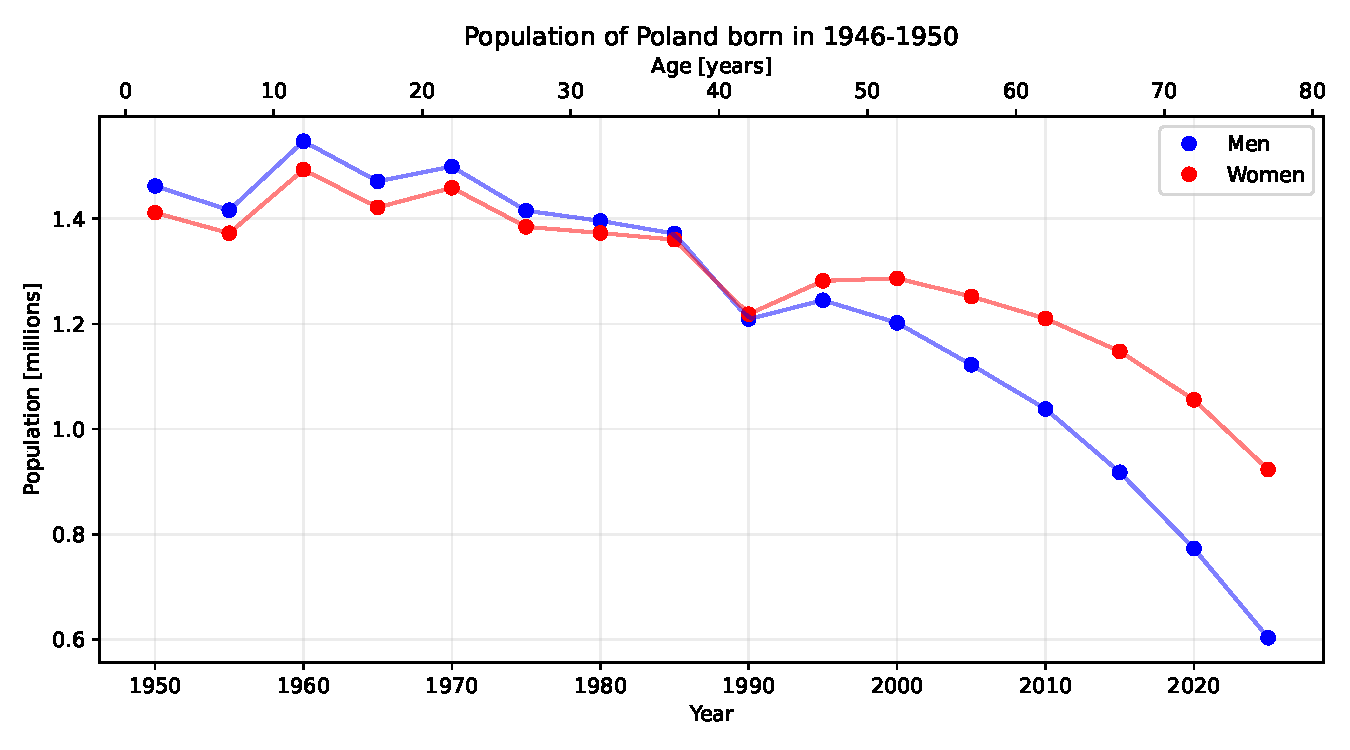
\includegraphics[width=0.8\linewidth]{images/task1.pdf}
		\caption{Population of men and women born in 1946--1950 as a function of the year (bottom axis) and of the age (top axis). The lines connecting the points are shown only to guide the eye.}
		\label{fig:task1}
	\end{figure}
	\FloatBarrier
		
	\section*{Task 2}
	
	\textit{Try to estimate median life expectancy (the age at which exactly 50\% of the initial population remains) for men and women born in 1946--1950. What problems do you encounter in your estimate?}
	
	\vspace{0.2cm}
	
	As initial population, the number of people in the age group $0$--$4$ in 1950 is used.
	The surviving fraction at age $a$ is then
	\begin{equation}
		f(a) = \frac{N(t)}{N(1950)},
		\label{eq:fraction}
	\end{equation}
	with $a$ and $t$ related by Eq.~\eqref{eq:age}.
	The median life expectancy $a_{1/2}$ is defined by the condition
	\begin{equation}
		f(a_{1/2}) = 0.5 .
		\label{eq:median}
	\end{equation}
	
	\subsection*{Men}
	
	For men the fraction drops below $0.5$ within the available data: $f_M = 0.529$ at $a_1 = 72$ (2020) and $f_M = 0.413$ at $a_2 = 77$ (2025).
	Between these two points, $f_M$ is approximated by the straight line through the points $(a_1, f_1)$ and $(a_2, f_2)$:
	\begin{equation}
		f_M(a) \simeq f_1 + \frac{f_2 - f_1}{a_2 - a_1}\,(a - a_1).
	\end{equation}
	Imposing $f_M(a_{1/2}) = 0.5$ and solving for the age gives
	\begin{equation}
		a_{1/2}^{M} = a_1 + \frac{0.5 - f_1}{f_2 - f_1}\,(a_2 - a_1)
		= 72 + \frac{0.5 - 0.529}{0.413 - 0.529}\cdot 5
		\simeq 73.2~\text{years}.
	\end{equation}
	
	\subsection*{Women}
	
	For women the fraction is still $f_F = 0.654$ in 2025, so the median life expectancy can only be obtained by extrapolating the data.
	Since the decrease of $f_F$ becomes faster with age, a parabola
	\begin{equation}
		f_F(a) = \alpha\, a^2 + \beta\, a + \gamma
	\end{equation}
	is fitted with the least-squares method (\texttt{scipy.optimize.curve\_fit}) to the last 5 points ($a = 57$--$77$, i.e.\ 2005--2025).
	The median life expectancy is then obtained by solving numerically (\texttt{scipy.optimize.brentq}) the equation
	\begin{equation}
		\alpha\, a^2 + \beta\, a + \gamma - 0.5 = 0
	\end{equation}
	in the interval $a \in [77,\, 100]$ years. The result is
	\begin{equation}
		a_{1/2}^{F} \simeq 83.8~\text{years}.
	\end{equation}
	Both results are shown in Figure~\ref{fig:task2}.
	
	\begin{figure}[!h]
		\centering
		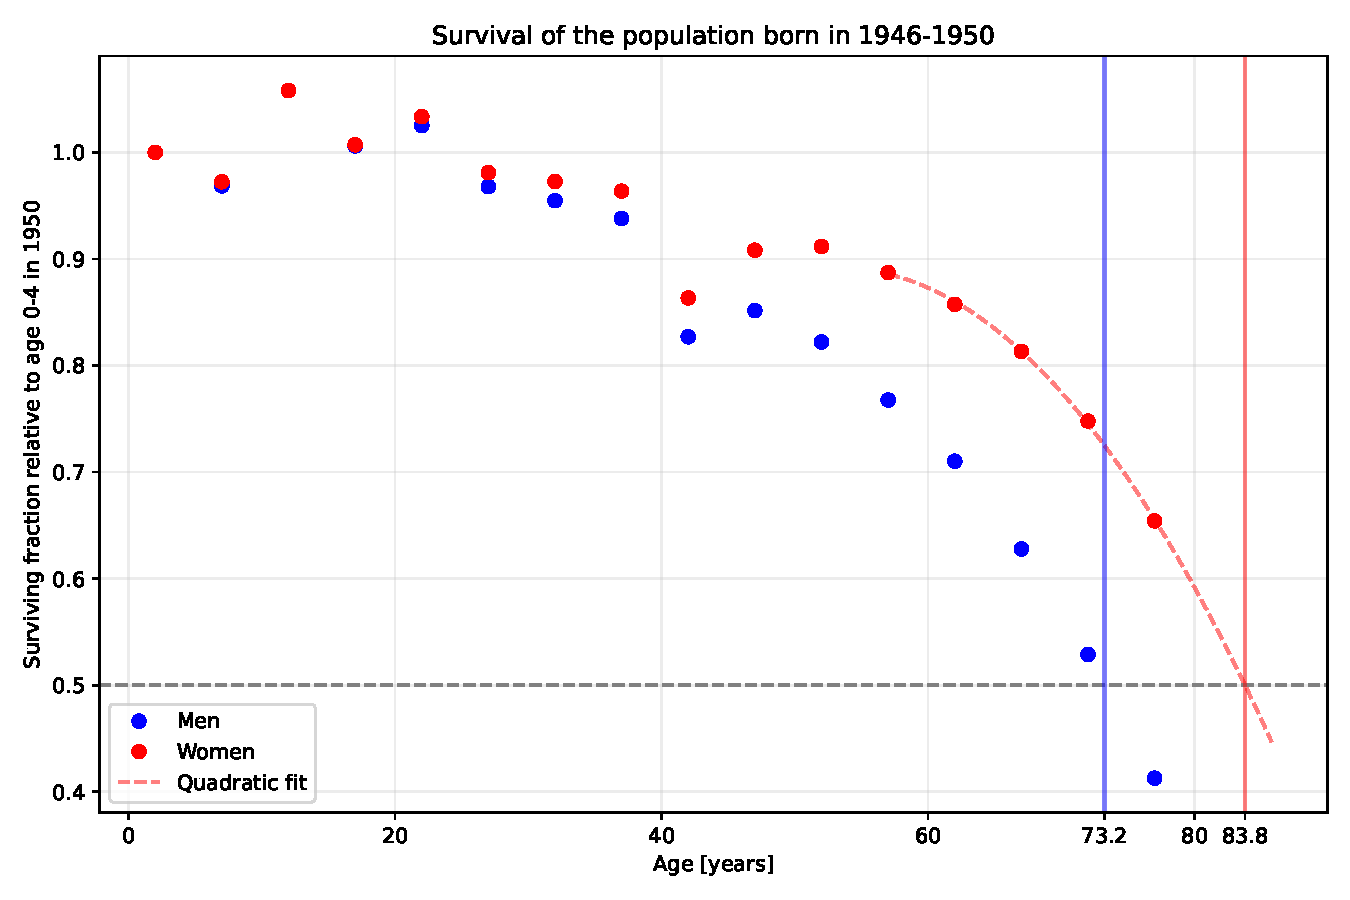
\includegraphics[width=0.8\linewidth]{images/task2.pdf}
		\caption{Surviving fraction of men and women born in 1946--1950, relative to the age group $0$--$4$ in 1950. The dashed red line is the quadratic fit used to extrapolate the data for women. The vertical lines mark the estimated median life expectancies.}
		\label{fig:task2}
	\end{figure}
	\FloatBarrier
	
	\subsection*{Problems of the estimate}
	
	\begin{itemize}
		\item \textbf{Extrapolation for women.} The 50\% threshold is not reached in the data for the female population, therefore the result depends on the chosen model and the number of data points used in the fit.
		The choice of the quadratic model is arbitrary, as is the choice of the number of data points to consider.
		
		
		\item \textbf{The population is not closed.} The surviving fraction exceeds 1. This is impossible for a closed group of people, whose number can only decrease.
		In fact, we are tracking the same group of people.
		The variations could be due to migration flows. The curve, therefore, does not describe mortality alone but is also influenced by people entering and leaving Polish territory. 
		
		\item \textbf{Definition of the initial population.} The data take into account only children who were still alive in 1950.
		Children born between 1946 and 1950 who died before 1950 are not included, so the actual initial population is larger.
		This means that the actual median life expectancy is lower than the estimated value.
		
	\end{itemize}
	
\end{document}
